

% To model the SRL as a MLN we define a set predicates to express our knowledge about the words of a sentences and the semantic relations. For example, the predicate \emph{lemma(p,l)} specifies the lemma $l$ for the word in the possition $p$. We say a predicate is grounded when it is in terms of atoms. Using our previous example, a grounded instance is \emph{lemma(4,play)} which means the lemma for the word in the fourth possition is \emph{play}. In ML, there are two types of predicates: observed and hidden. The observed predicates represent the knowledge we are certain about and the hidden represent the knowledge we are interested to know about. In the SRL task, we are interested in the predicates which represent the semantic relations. 

We define five hidden predicates for the three stages of the task. Figure \ref{fig:achitecture} illustrates these predicates and the stage they belong to. 

For predicate identification, we use the predicates \emph{isPredicate} and \emph{sense}. \emph{isPredicate(p)} indicates that the word in the position $p$ is an SRL predicate while \emph{sense(p,e)} signals that predicate in position $p$ has the sense $e$. %\footnote{The sense corresponds to the label after the  ``.'' symbol in a roleset.}. 

For argument identification, we use the predicates \emph{isArgument} and \emph{hasRole}. The atom \emph{isArgument(a)} signals that the word in the position $a$ is a SRL argument of some (unspecified) SRL predicate while \emph{hasRole(p,a)} indicates that the token at position $a$ is an argument of the predicate in position $p$. 

Finally, for the argument classification stage we define the predicate \emph{role}. Here \emph{role(p,a,r)} corresponds to the decision that the argument $a$ has the role $r$ with respect to the predicate $p$.

% There is a potential problem of coupling the predicates. For instance, the predicate $hasRole(p,a)$ could be true, but there is not guaranty that the predicate $predicate(p)$ is. This situation would lead to arguments without SRL predicates. In the following, subsections we explain how we can constrain these two predicates to be couple using the FOL formulae of the MLN model. Aditionally, we show how we can relate our knowledge from the words with the predicates for the SRL task.


\begin{figure}
\begin{center}
    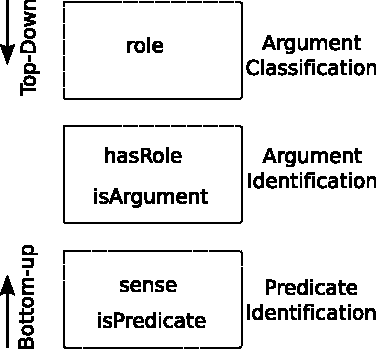
\includegraphics[scale=.80]{TaskArchitecture}
\end{center}
\caption{MLN hidden predicates divided in stages}
\label{fig:achitecture}
\end{figure}

